%!TEX root = ./fuzzylite-1.01.tex
\chapter{The Model}
	This chapter is devoted to explain \fl\ by means of a class diagram based on UML. For a better comprehension, it is divided in five groups: Fuzzy operations, Linguistic variables and terms, Linguistic terms, Fuzzy rules, Fuzzy engine, and Fuzzy exceptions. It is important to mention that all classes related to \fl\ are inside the namespace \texttt{fl}.
	
	\section{Fuzzy operations}
		Figure~\ref{f:fuzzy-ops} shows the class diagram for this group. The classes that can be seen in it are briefly explained in the following sections.
		
		\begin{landscape}
			

		\begin{figure}[ht]
			\centering
			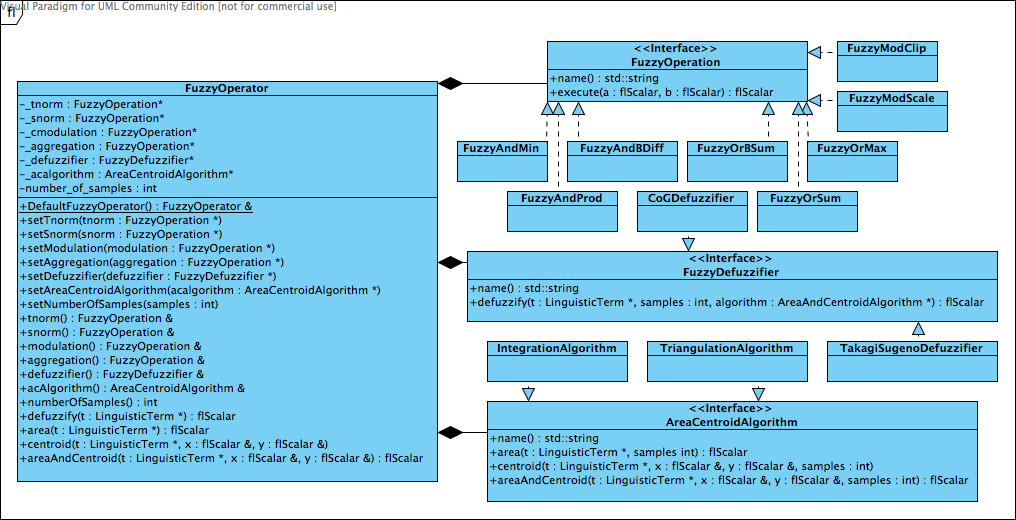
\includegraphics[scale=0.7]{./figures/fuzzy-ops.png}
			\caption{Class diagram: Fuzzy operations}
			\label{f:fuzzy-ops}
		\end{figure}
				\end{landscape}
		
		\subsection{\texttt{FuzzyOperator}}
			\texttt{FuzzyOperator} centralizes all the operations that can be performed in the fuzzy system. It contains the type of T-Norms, S-Norms, modulation, aggregation, defuzzification methods, algorithms for computing the area and centroid of any linguistic term, and the number of samples that are drawn from any linguistic term to be used by the algorithm. 
			
			This class has an static default \texttt{FuzzyOperator} instance that can be obtained using the method \texttt{fl::FuzzyOperator::DefaultFuzzyOperator()} anywhere and anytime. The defaults for this operator are the following

			\begin{multicols}{2}
			\begin{itemize}[nolistsep]
				\item \textbf{T-Norm:} \texttt{FuzzyAndMin}.
				\item \textbf{S-Norm:} \texttt{FuzzyOrMax}.
				\item \textbf{Modulation:} \texttt{FuzzyModClip}.
				\item \textbf{Aggregation:} \texttt{FuzzyOrMax}.
				\item \textbf{Defuzzifier:} \texttt{CoGDefuzzifier}.
				\item \textbf{Algorithm:} \texttt{TriangulationAlgorithm}.
				\item \textbf{Number of samples:} 100.
			\end{itemize}
			\end{multicols}
	
	These defaults may be changed at any moment from anywhere, but consider that this is an instance that is shared among all instances from many classes, so be careful about changing these values. Nevertheless, if you need to, you may use different instances among all those classes composed by \texttt{FuzzyOperator}. 
	
	\subsection{\texttt{FuzzyOperation}}
		This is the interface shared by all T-Norms, S-Norms, and methods for modulation and aggregation. If you want to implement your own operations, you may do so by implementing  this interface. The operations included in \fl\ are:
		
		\begin{itemize}
			\item T-Norm: minimum (\texttt{FuzzyAndMin}), product (\texttt{FuzzyAndProd}), and bounded difference (\texttt{FuzzyAndBDiff}).
			\item S-Norm: maximum (\texttt{FuzzyOrMax}), sum (\texttt{FuzzyOrSum}), bounded sum (\texttt{FuzzyOrBSum}).
			\item Modulation: clipping (\texttt{FuzzyModClip}), scaling (\texttt{FuzzyModScale}).
			\item Aggregation: maximum (\texttt{FuzzyOrMax}), sum (\texttt{FuzzyOrSum}), bounded sum (\texttt{FuzzyOrBSum}).
		\end{itemize}
		
	\subsection{\texttt{FuzzyDefuzzifier}}
		This is the interface shared by all defuzzifiers. If you want to implement a different defuzzifier, you may do so by implementing this interface. The defuzzifiers included in \fl\ are: Centre of Gravity (\texttt{CoGDefuzzifier}) for Mamdani rules, and \texttt{TakagiSugenoDefuzzifier} for Takagi-Sugeno rules.
		
	\subsection{\texttt{AreaAndCentroidAlgorithm}}
		This is an interface used for computing the area and centroid of linguistic terms. The algorithms included in \fl\ are: \texttt{TriangulationAlgorithm} which is a triangulation algorithm appropriate for terms that can be easily triangulated, and \texttt{IntegrationAlgorithm} which is a regular integration algorithm. The algorithm should be chosen according to the shape of the fuzzy partitions. You may also create your own algorithm by implementing this interface.
		
		
	\section{Linguistic variables and terms}
		Figure~\ref{f:linguistics} shows the class diagram for the linguistic variables and terms included in \fl. 
		
		\begin{landscape}
			

		\begin{figure}[ht]
			\centering
			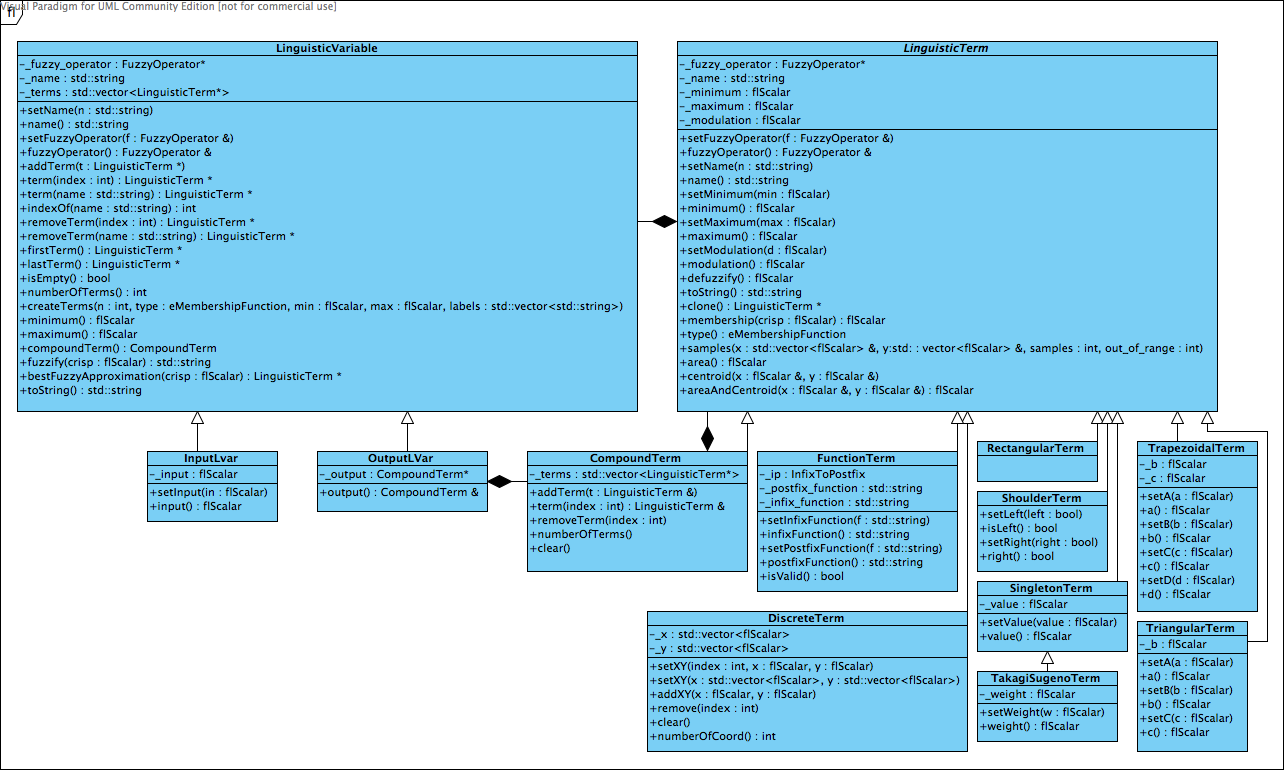
\includegraphics[scale=0.55]{./figures/fuzzy-linguistic.png}
			\caption{Class diagram: Linguistic variables and terms}
			\label{f:linguistics}
		\end{figure}
		\end{landscape}		
		\subsection{\texttt{LinguisticVariable}}
			Linguistic variables are composed of a vector of \texttt{LinguisticTerm}s. This is an abstract class that is used as base for input variables (\texttt{InputLVar}) and output variables (\texttt{OutputLVar}). Each input variable has an input value that should be the input received by the system, and each output variable has a compound linguistic term composed by all the linguistic terms added by the activation of the different rules given the input values of the input variables and their respective processing.
			
		\subsection{\texttt{LinguisticTerm}}
			Linguistic terms, also known as fuzzy partitions, define the shape of each label. Each linguistic term has a minimum and maximum that are used to define the limits of the area it covers. Several linguistic terms are included in \fl:

			\begin{itemize}
				\item \texttt{TriangularTerm}: is the well known triangular term, it is defined by its three vertices $a$, $b$, and $c$, where $a$ and $c$ are wrappers of \texttt{minimum()} and \texttt{maximum()}, respectively.
				\item \texttt{RectangularTerm}: is a simple rectangular term delimited by the minimum and maximum of its parent class \texttt{LinguisticTerm}.
				\item \texttt{TrapezoidalTerm}: defines a trapezoid by its four vertices $a$, $b$, $c$, and $d$, where $a$ and $d$ are wrappers of \texttt{minimum()} and \texttt{maximum()}, respectively.
				\item \texttt{SingletonTerm}: defines a singleton for the value $v$ delimited by $v - \delta_{low}$ and $v + \delta_{hi}$ where $\delta_{low}$ and $\delta_{hi}$ are very small values in order to be able to create samples of this term.
				\item \texttt{ShoulderTerm}: defines a trapezoid that extends to $\pm\infty$  depending on whether it is left ($-\infty$) or right ($+\infty$).
				\item \texttt{DiscreteTerm}: is a term composed of a vector of $(x,y)$ coordinates.  It is important to note that when sampling this type of term, the result of \texttt{membership(flScalar crisp)} is the value of $y$ for the closest $x$ given the value of \texttt{crisp}.
				\item \texttt{FunctionTerm}: is a term that is defined as a function $f(x)$ which accepts several mathematical and trigonometrical operations over a given function, for example: \texttt{setInfixFunction( "(sin x) / x" )}. It is \emph{very} important to remark that the parser used to parse infix functions may not function as expected (e.g. $\sin (x) / x$ is different of $(\sin x) / x$, the latter one gives the result one expects). When in doubt, test your expression by converting it to postfix.
				\item \texttt{CompoundTerm}: is a term composed of a list of \texttt{LinguisticTerm}s. This is used in \texttt{OutputLVar} in order to aggregate all the linguistic terms that were added by the activation of rules, but it may be used as well to create more complex partitions.
				\item \texttt{TakagiSugenoTerm}: is a term used when dealing with \texttt{TakagiSugenoRule}s, it extends from \texttt{SingletonTerm} so it has a value, and it  includes a \texttt{weight} as well, both necessary for this kind of system.
			\end{itemize}

			Finally, figure~\ref{f:lterms} shows examples of the linguistic terms, obtained by printing the window from the GUI developed for \fl.

		\begin{figure}[ht]
			\centering
			\subfigure[\texttt{TriangularTerm}] 
			{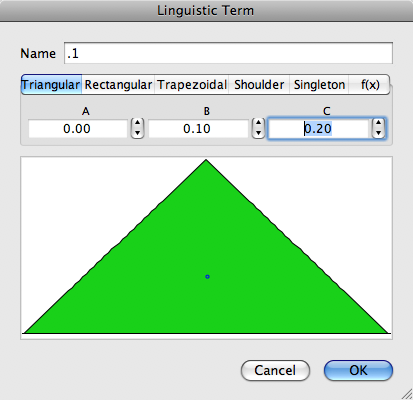
\includegraphics[scale=0.3]
			{./figures/ft-triangular.png}} 
			\subfigure[\texttt{RectangularTerm}]
			{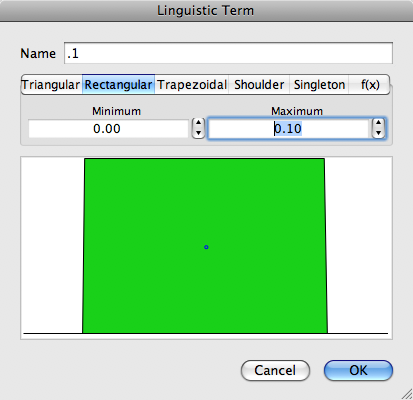
\includegraphics[scale=0.3]
			{./figures/ft-rectangular.png}}
			\subfigure[\texttt{TrapezoidalTerm}]
			{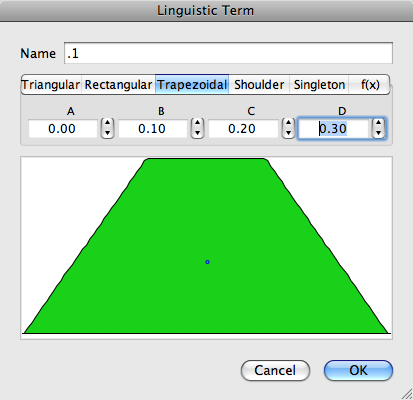
\includegraphics[scale=0.3]
			{./figures/ft-trapezoidal.png}} \\
			\subfigure[\texttt{SingletonTerm}]
			{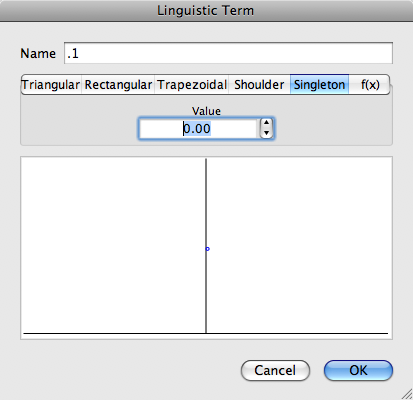
\includegraphics[scale=0.3]
			{./figures/ft-singleton.png}} 
			\subfigure[\texttt{ShoulderTerm} (left)] 
			{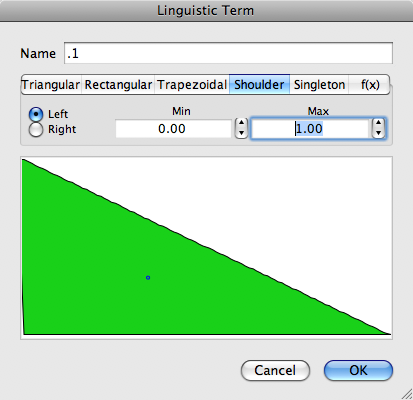
\includegraphics[scale=0.3]
			{./figures/ft-lshoulder.png}} 
			\subfigure[\texttt{ShoulderTerm} (right)]
			{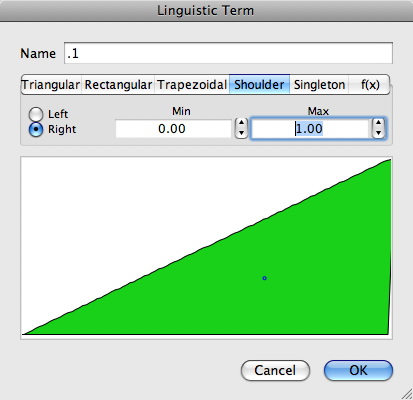
\includegraphics[scale=0.3]
			{./figures/ft-rshoulder.png}}\\
			\subfigure[\texttt{FunctionTerm}]
			{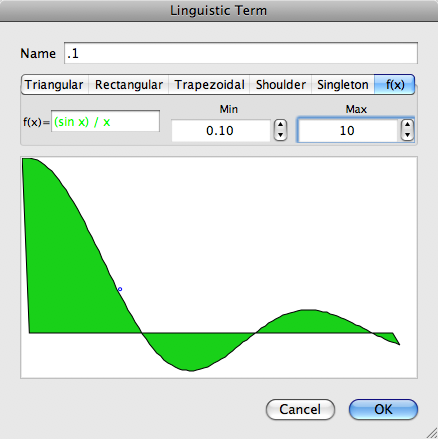
\includegraphics[scale=0.3]
			{./figures/ft-function.png}}
			\subfigure[Triangular partitions]
			{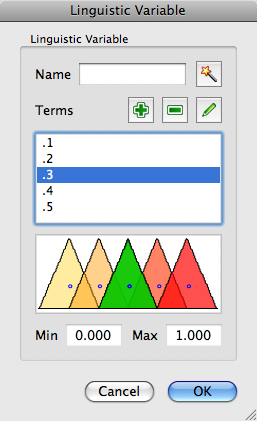
\includegraphics[scale=0.4]
			{./figures/ft-partition-1.png}}
			\subfigure[Triangular + Shoulder partitions]
			{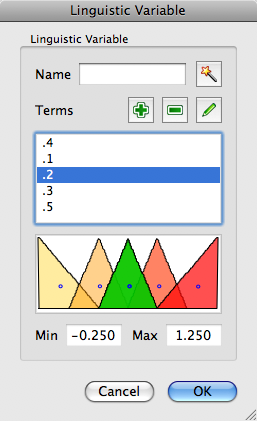
\includegraphics[scale=0.4]
			{./figures/ft-partition-2.png}}
			\caption{Linguistic Terms}
			\label{f:lterms}
		\end{figure}
		
	\section{Fuzzy rules}
		Figure~\ref{f:fuzzy-rules} shows the class diagram for fuzzy rules and all its related classes included in \fl.
		
		\begin{landscape}
			\begin{figure}[ht]
				\centering
				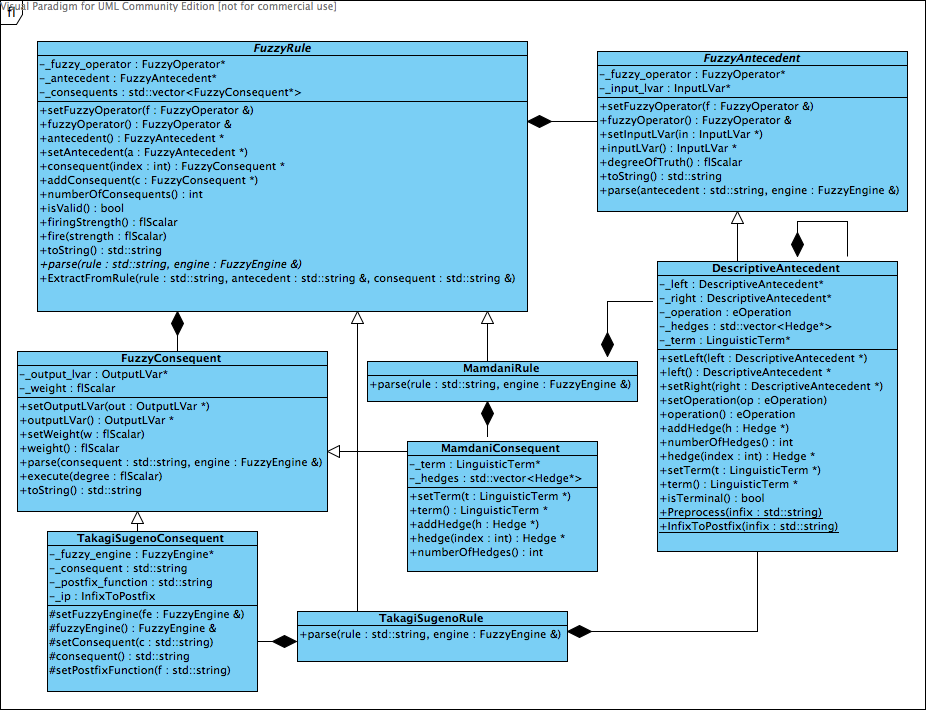
\includegraphics[scale=0.58]{./figures/fuzzy-rules.png}
				\caption{Class diagram: Fuzzy rules}
				\label{f:fuzzy-rules}
			\end{figure}
		\end{landscape}
		
		\subsection{\texttt{FuzzyRule}}
			This abstract class is the base for \texttt{MamdaniRule}s and \texttt{TakagiSugenoRule}s. It is composed by an antecedent (\texttt{FuzzyAntecedent}) and a list of consequents (\texttt{FuzzyConsequent}s). There are two methods that are worth mentioning here: \texttt{firingStrength()} which determines the activation degree of the rule given the inputs in the \texttt{InputLVar}s, and \texttt{fire( flScalar d )} which fires the rule with a degree $d$. When firing the rule, the consequents are modulated according to $d$ and then added to the \texttt{OutputLVar}s with the respective weight of the rule. It is also important to remark that parsing the rules is case-sensitive.
			
		\subsubsection{\texttt{FuzzyAntecedent} and \texttt{FuzzyConsequent}}
			These abstract classes represent the antecedent and consequent of a rule, respectively. \texttt{FuzzyAntecedent} has a pointer to the input variable to which it is related in order to access the value of the respective \texttt{InputLVar}, similarly, \texttt{FuzzyConsequent} has a pointer to the output variable to which it is related in order to aggregate the respective modulated linguistic term to the output.
			
			
		\subsubsection{\texttt{DescriptiveAntecedent}}
			This class is based on \texttt{FuzzyAntecedent} and it is a red-black tree that relates two propositions with an operator, for example, \texttt{input-1} \textbf{is} \texttt{LOW} \textbf{and}  \texttt{input-2} \textbf{is} \texttt{GOOD} is separated into a left antecedent (\texttt{input-1} \textbf{is} \texttt{LOW}), an operator (\textbf{and}),   and a right antecedent (\texttt{input-2} \textbf{is} \texttt{GOOD}). Given the recursion of  this model, it is possible to create rules of any depth, as it is evaluated bottom-up. This is the class used by \texttt{MamdaniRule} and \texttt{TakagiSugenoRule}.
		
		\subsubsection{\texttt{Hedge}}
			Hedges are modifiers of the propositions (antecedent) and actions (consequent). All hedges must implement the interface \texttt{Hedge}, and must be included when configuring the \texttt{FuzzyEngine}. \fl\ includes four hedges: not (\texttt{HedgeNot}), somewhat (\texttt{HedgeSomewhat}), very (\texttt{HedgeVery}), any (\texttt{HedgeAny}). In order to use \texttt{HedgeAny}, it is necessary to include a \emph{dummy} linguistic term to comply with the general form of the rules (i.e. \emph{input-1} \textbf{is} \texttt{any} \texttt{LOW}); this hedge will always return 1.0, so it does not matter the linguistic term as long as it is within the linguistic variable used. Figure~\ref{f:hedges} shows the class diagram regarding hedges.
			
			\begin{figure}[ht]
				\centering
				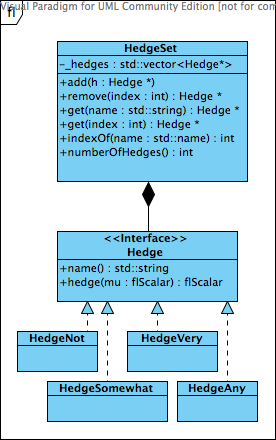
\includegraphics[scale=0.65]{./figures/fuzzy-hedges.png}
				\caption{Class diagram: Hedges}
				\label{f:hedges}
			\end{figure}
		
		\subsubsection{\texttt{MamdaniRule} and \texttt{TakagiSugenoRule}}
			These classes represents the type of rules of a system based on Mamdani's rules, and the one based on Takagi-Sugeno rules, respectively. They extend the abstract class \texttt{FuzzyRule} by implementing the \texttt{parse()} method accordingly. Both classes use \texttt{DescriptiveAntecedent} as the antecedent of the rule, but differ in the consequent: \texttt{MamdaniRule} uses \texttt{MamdaniConsequent}, and \texttt{TakagiSugenoRule} uses \texttt{TakagiSugenoConsequent}.
			
		\subsubsection{\texttt{MamdaniConsequent} and \texttt{TakagiSugenoConsequent}}
			The consequent of a Mamdani rule is of the form: \texttt{OutputLVar} \textbf{is} [\texttt{Hedge}$^*$] \texttt{LinguisticTerm}, where [\texttt{Hedge}$^*$] means that none or many hedges may be included.
			
			Conversely, the consequent of a Takagi-Sugeno rule is of the form \texttt{OutputLVar}=\{\emph{expression}\}, where \emph{expression} is a mathematical expression that may include references to the values of the \texttt{InputLVar}s, in which case the name of the input variable is used (e.g. "... f\_x=0.5 * input-1 + (sin input-2)"). This implementation also allows to include previously computed outputs, in which case the name of the output should be used instead.
	
	\section{Fuzzy engine}
		The class diagram for this group can be seen in figure~\ref{f:fuzzy-engine}. It contains the class \texttt{FuzzyEngine} which is composed by a \texttt{FuzzyOperator}, a vector of \texttt{RuleBlock}s which contain the \texttt{FuzzyRule}s, a \texttt{HedgeSet} that contains the hedges registered in the engine, and a vector of \texttt{InputLVar}s and \texttt{OutputLVar}s for input and output variables (respectively).
		
		The \texttt{FuzzyEngine} class contains the whole fuzzy control system. The only methods which might require a bit of explanation are \texttt{process( bool )}, and \texttt{process(int, bool)}. The former receives a boolean parameter that defaults to \texttt{true} and (if true) clears the output of all the output variables. The latter receives an \texttt{int} parameter that determines the index of the \texttt{RuleBlock} to be fired, and a \texttt{bool} that defaults to \texttt{true} which defines whether to clear the output of the output variables.
		
		\begin{landscape}
		\begin{figure}[ht]
			\centering
			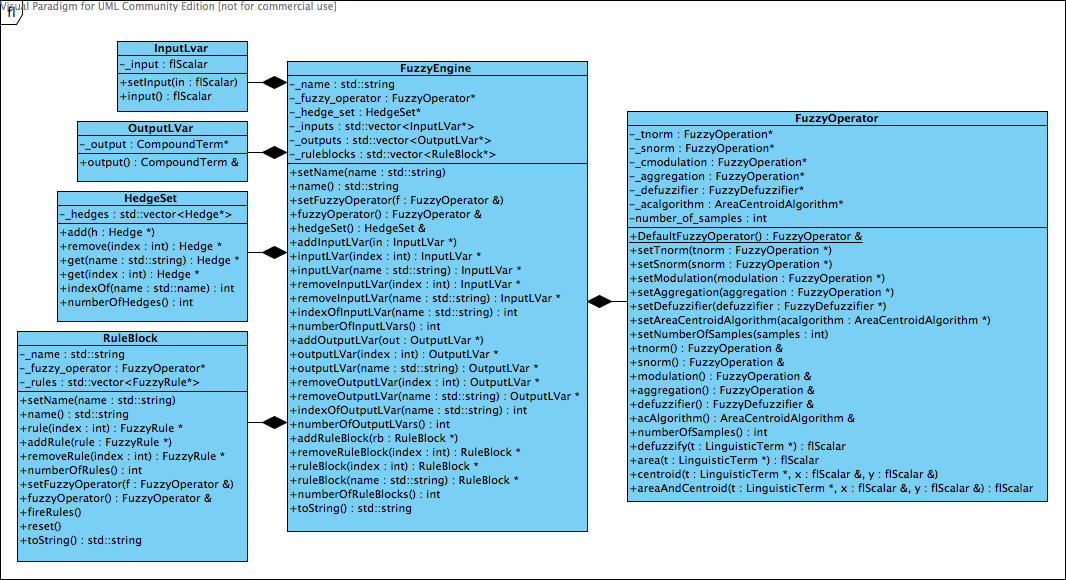
\includegraphics[scale=0.65]{./figures/fuzzy-engine.png}
			\caption{Class diagram: Fuzzy engine}
			\label{f:fuzzy-engine}
		\end{figure}
		\end{landscape}
	
	\section{Fuzzy exceptions}
		This group contains some exceptions that are used within several classes of \fl. The class \texttt{FuzzyException} extends the \texttt{std::exception} of the Standard Template Library (STL), and adds additional methods. The other classes derived from \texttt{FuzzyException} also contain some static methods to help a bit with the programming. There is not much to say about these exceptions, except to take a look at the code when using them to become familiar. Figure~\ref{f:fuzzy-exceptions} shows the class diagram for this group.
		
		
	\begin{figure}[ht]
		\centering
		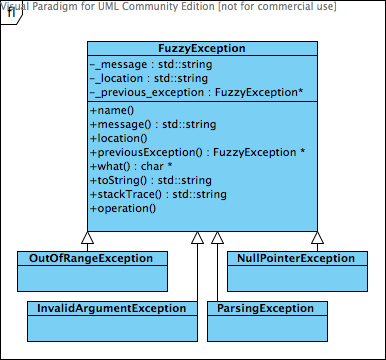
\includegraphics[scale=0.65]{./figures/fuzzy-exceptions.png}
		\caption{Class diagram: Fuzzy exceptions}
		\label{f:fuzzy-exceptions}
	\end{figure}
	
	
